\documentclass{article}

% Packages for title page
\usepackage{graphicx} % For including images
\usepackage{titling} % For modifying the title
\usepackage{datetime} % For including date and time
\usepackage{geometry}
 \geometry{
 a4paper,
 left=20mm,
 top=20mm,
 }

% Packages for table of contents
\usepackage{tocloft} % For modifying the table of contents

% Packages for main content
\usepackage{lipsum} % For generating placeholder text
\usepackage{hyperref} % For creating hyperlinks

% Set up title page
\pretitle{\begin{center} \LARGE 
\includegraphics[width=0.5\linewidth]{tulogo.png}\\[\bigskipamount]\end{center}}
\posttitle{}

\title{ \begin{center} \LARGE Vehicle Accident Prevention System (VAPS) \end{center} }
\author{\\ \\Team Members: 
\\
\\
\\
Aman Kumar EEB20035\\
Apoorv Krishan EEB20034\\
Shabnam Ajaj EEB20025\\
Vicky Kumar EEB20043\\}
\date{}


% Set up table of contents
\setlength\cftbeforesecskip{0.5em} % Space between sections in the table of contents

\begin{document}

\maketitle
\newpage
\tableofcontents

\newpage

\section{Objective}
Our proposed project focuses on addressing the alarming issue of vehicle accidents, with a particular emphasis on heavy vehicles. The primary cause of these accidents is driver negligence, which most commonly manifests in the form of drowsy driving and driving under the influence of alcohol. The consequences of such accidents can be catastrophic, causing loss of life, property damage, and financial burden.
\\
\\
Therefore, our project aims to provide a comprehensive solution that not only tackles the problem of accidents but also streamlines the logistics process. We envision an end-to-end system that incorporates cutting-edge technologies to solve the problem. By leveraging these technologies, we can develop a solution that can accurately monitor drivers' behaviour and alert them in real-time if they exhibit signs of drowsiness or impairment.
\\
\\
Furthermore, our solution will incorporate intelligent law enforcement helping tools to help maintain the law and order on the roads. Our ultimate goal is to make the roads safer for everyone while improving the bottom line for logistics companies.

\section{Background}
The problem of vehicle accidents due to driver negligence, specifically drowsy and drunk driving, has become a growing concern worldwide. These accidents result in significant loss of life, property damage, and financial burden. Despite the implementation of strict laws and regulations, many drivers continue to engage in these unsafe practices, leading to preventable accidents.
\\ \\
Current solutions to address this problem, such as random breath testing and driver education programs, have limitations in terms of effectiveness and scalability. Furthermore, these solutions do not provide real-time feedback to drivers, leaving room for human error and increasing the risk of accidents.
\\ \\
To address these issues, we propose the use of Arduino and sensors to detect drowsiness and drunk driving in real time. This solution has the potential to significantly reduce the number of accidents caused by driver negligence, making driving safer and more efficient. However, the development of such a system requires careful consideration and planning to ensure that it is reliable, accurate, and cost-effective.
\\ \\
Therefore, the problem statement for our proposed project is to design and develop a comprehensive system using Arduino and sensors that can accurately detect drowsiness and drunk driving in real-time, providing feedback to drivers to prevent accidents caused by driver negligence.

\section{Methodology}
The design and development of the solution can be divided into two parts: Hardware development and Software Development. 
\\ \\ 
The two parts are the essential parts for the working of the entire solution.  While the hardware part is essential for the interaction of the system with humans (driver) while the software part is the decision-maker and background assisting part of the system, which helps to streamline the solution as well as make it user-friendly and cheap. 

\begin{figure}[ht]

\centering
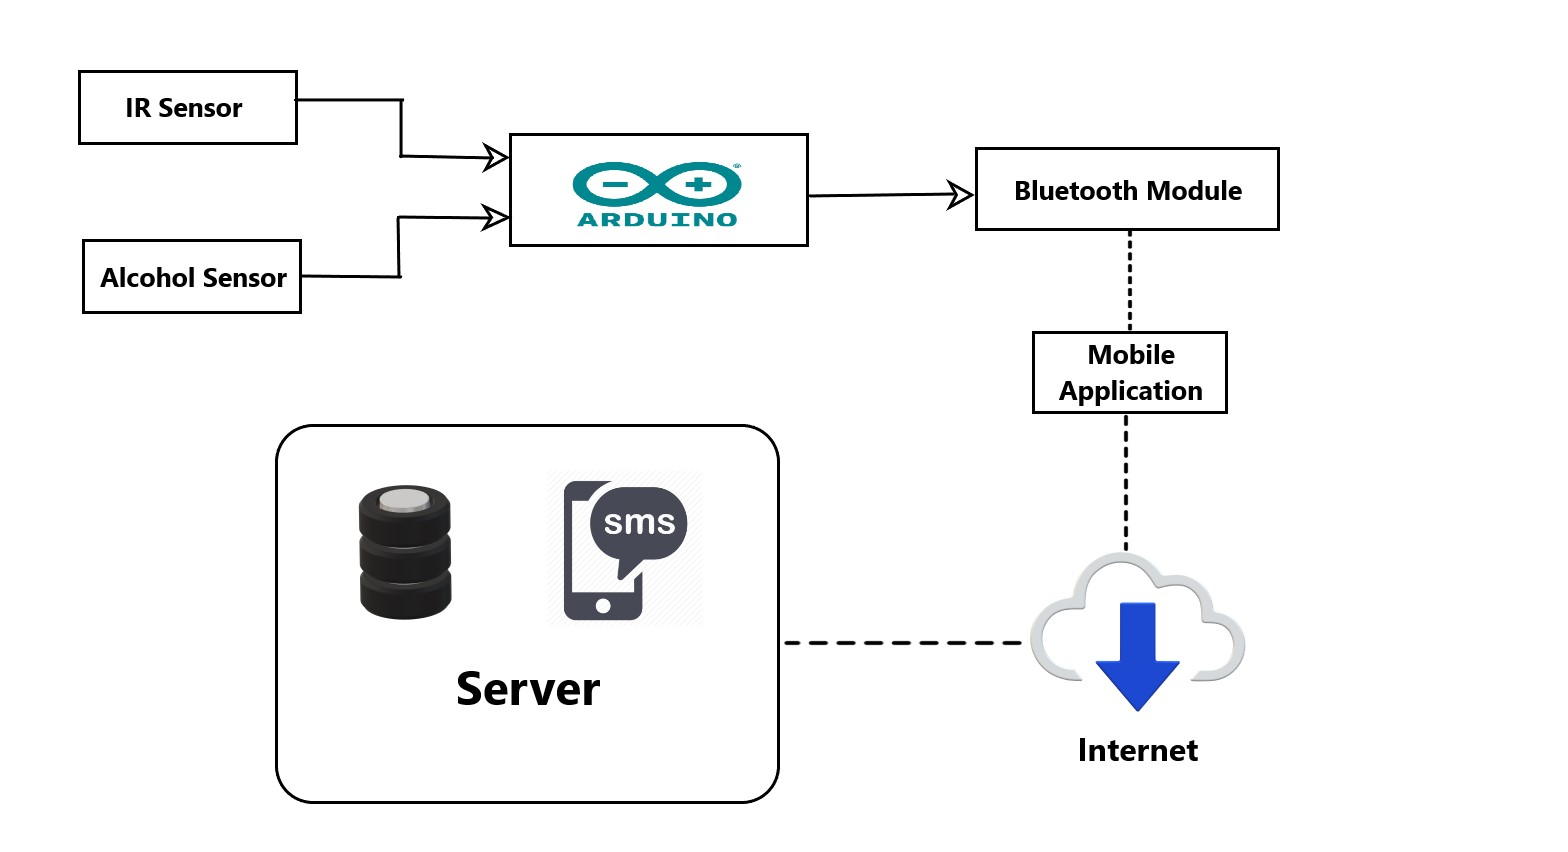
\includegraphics[width=\textwidth]{eld_report.jpg}
\caption{System Design of the proposed solution.}

\end{figure}

\subsection{Hardware Development}
The development of the hardware for the proposed solution includes the making of a spectacle to track drowsiness and alcohol consumption by the user (driver). This developed hardware solution will be employing a low-power, open-source device Arduino for onboard data processing, an infrared sensor (IR) for eye tracking and sleep detection, and an MQ3 Alcohol sensor for alcohol detection on board. The sensors will be able continuously to track the driver for any anomaly and detect sleep or sleep-like symptoms along with the consumption of alcohol. \\ \\

This entire hardware assembly will be mounted on a glass frame for demonstration purposes but can also be made into a final product similarly. The Arduino will be connected to an HC-05 Bluetooth module that can be connected to the user's smartphone device via Bluetooth. \\

Along with that, the Arduino can be programmed to trigger a separate system that can reduce the vehicle speed as well as switch on the hazard lights to indicate the potential problem with the vehicle on the road. 

\subsection{Software Development}
As important is the hardware part in our proposed solution for the detection of anomalies in the driver behaviour, the software part is also similarly important to make this proposed solution cheap and effective. \\ \\ 
The Bluetooth module connected via Bluetooth to the user's smartphone device would be communicating with the app we will develop. This app functions as a service installed on the device and would constantly wait for the anomaly signal. As soon as the anomaly signal is detected, the app will send the Geo-location of the vehicle to our web server which will operate on the web and listen for such data. \\

The web server then starts its function by trying to calculate the distance to the nearest Highway Patrol Vehicle or Police Station and will alert them through a mode of communication, for example, SMS, with the location of the affected vehicle. This helps to enforce the law and order in the area more effectively. \\

However, this will cause the logistics to suffer and thus the proposed solution is that the web server will also send a message to the logistics company regarding the situation. This helps in a way that due to the reception of the information on time, the company can deploy a secondary driver to take over the charge of the vehicle and logistics, while also helping to make the legal proceedings smooth. 
% \section{Results}
% \lipsum[4]

% \section{Discussion}
% \lipsum[5]

\section{Conclusion}
The proposed solution is expected to perform as designed and possess great potential to reduce the number of accident that happens due to problems discussed here like the sleepy driver problem and drunk driver problem. Not only it's expected to maintain the safety of the driver and others on the road, but it's also expected to help the police to maintain the law and order on the road while keeping the logistics system safe from point failure. 

% Add references section
% \section*{References}
% \addcontentsline{toc}{section}{References}

% Add references here

\end{document}
